\documentclass[10pt, conference]{IEEEtran}
\usepackage{amssymb,amsthm,amscd,bm}
\usepackage[cmex10]{amsmath}

\usepackage{listings}
\lstset{language=C++, basicstyle=\normalsize}

\usepackage{graphicx}

\usepackage[tight,footnotesize]{subfigure}

\usepackage[named]{algo}

\usepackage{url}

\usepackage{tabularx}

%\usepackage{times}
%\usepackage{expdlist}

\newcommand{\ib}[1]{\textbf{#1}}
\newcommand{\gC}{\ib{C}}
\newcommand{\gD}{\ib{D}}
\newcommand{\gF}{\ib{F}}
\newcommand{\gG}{\ib{G}}
\newcommand{\gH}{\ib{H}}
\newcommand{\gK}{\ib{K}}
\newcommand{\gR}{\ib{R}}
\newcommand{\gL}{\ib{L}}
\newcommand{\gO}{\ib{O}}
\newcommand{\gV}{\ib{V}}
\newcommand{\gRs}{\gR_s}
\newcommand{\gRx}{\gR_{\times}}
\newcommand{\gI}{\ib{I}}
\newcommand{\gN}{\ib{N}}
\newcommand{\gP}{\ib{P}}
\newcommand{\gf}{\ib{f}}
\newcommand{\gp}{\ib{p}}
\newcommand{\gs}{\ib{s}}
\newcommand{\ga}{\ib{a}}
\newcommand{\gb}{\ib{b}}
\newcommand{\gc}{\ib{c}}
\newcommand{\gd}{\ib{d}}

\newcommand{\inrhd}{i_{\nrhd}}
\newcommand{\inlhd}{i_{\nlhd}}
\newcommand{\isim}{i_{\sim}}

\newcommand{\cR}{\mathcal{R}}
\newcommand{\cRs}{\cR_s}
\newcommand{\cRx}{\cR_{\times}}

\newcommand{\nT}{\mathbb{T}}
\newcommand{\Nat}{\mathbb{N}}

\newcommand{\gFs}{\gF^*}
\newcommand{\gFu}{\gF^{\cup}}

\newcommand{\executes}{\textit{executes}}
\newcommand{\pure}{\textit{pure}}
\newcommand{\params}{\textit{params}}
\newcommand{\func}{\textit{func}}
\newcommand{\adj}{\textit{adj}}
\newcommand{\any}{\textit{any}}
\newcommand{\isPrim}{\textit{isPrimitive}}
\newcommand{\isSol}{\textit{isSolution}}
\newcommand{\isPartSol}{\textit{isPartSolution}}
\newcommand{\fixed}{\textit{fixed}}
\newcommand{\children}{\textit{children}}
\newcommand{\type}{\textit{type}}
\newcommand{\merge}{\textit{merge}}
\newcommand{\adjacent}{\textit{adjacent}}
\newcommand{\parents}{\textit{parents}}
\newcommand{\loc}{\textit{loc}}
\newcommand{\offset}{\textit{offset}}
\newcommand{\vtable}{\textit{vtable}}

\newcommand{\positive}{\textit{positive}}
\newcommand{\sequence}{\textit{sequence}}
\newcommand{\nlhd}{\ntriangleleft}
\newcommand{\nrhd}{\ntriangleright}

\newcommand{\bs}{$\blacksquare$}

%\newtheorem{statement}{Statement}
%\newtheorem{rulez}{Rule}
%\newtheorem{lemma}{Lemma}
%\newtheorem{theorem}{Theorem}
%\newtheorem{cmr}{Consistency maintenance rule}

\newcommand{\listingsize}{\normalsize}

\renewenvironment{itemize}{
    \begin{list}{\labelitemi}{\leftmargin=1.0em \itemindent=-0.4em \itemsep=-\parsep}
}{
	\end{list}
}

\newcounter{xcounter}
\renewenvironment{enumerate}{
    \begin{list}{\arabic{xcounter})}{\usecounter{xcounter} \leftmargin=1.5em \itemindent=-0.85em \itemsep=-\parsep}
}{
	\end{list}
}

\newcounter{rulecounter}
\newenvironment{rulez}{
    \noindent
    \textbf{\addtocounter{rulecounter}{1}Rule \arabic{rulecounter}.}
    \it
}{
	\em
}


\pagestyle{empty}
%\pagestyle{plain}  %%% TODO FOR CAM-READY?

\begin{document}

\title{Reconstruction of Class Hierarchies for Decompilation of C++ Programs}

\author{
    \IEEEauthorblockN{
        A. Fokin\IEEEauthorrefmark{1},
        K. Troshina\IEEEauthorrefmark{2} and
        A. Chernov\IEEEauthorrefmark{3}
    }
    \IEEEauthorblockA{
        \IEEEauthorrefmark{1}
        Computational Math. and Cybernetics Dept., Moscow State University,\\
        Leninskie Gory, Moscow, Russia\\
        Email: apfokin@gmail.com
    }
    \IEEEauthorblockA{
        \IEEEauthorrefmark{2}
        Institute for System Programming, Russian Academy of Sciences,\\
        25, Alexander Solzhenitsyn st., Moscow, Russia\\
        Email: katerina@ispras.ru
    }
    \IEEEauthorblockA{
        \IEEEauthorrefmark{3}
        Computational Math. and Cybernetics Dept., Moscow State University,\\
        Leninskie Gory, Moscow, Russia\\
        Email: cher@unicorn.cmc.msu.ru
    }
}

\maketitle
%\thispagestyle{plain}

\begin{abstract}
This paper presents a method for automatic reconstruction of
polymorphic class hierarchies from the assembly code obtained by
compiling a C++ program.
If the program is compiled with run-time type information (RTTI),
class hierarchy is reconstructed via analysis of RTTI structures.

In case RTTI structures are missing in the assembly, a technique
based on the analysis of virtual function tables, constructors and
destructors is used.

A tool for automatic reconstruction of polymorphic class hierarchies
that implements the described technique is presented.
This tool is implemented as a plugin for IDA Pro Interactive Disassembler.
Experimental study of the tool is provided.
\end{abstract}

\begin{IEEEkeywords}
decompilation; reverse engineering; C++; class hierarchy reconstruction;
\end{IEEEkeywords}





\section{Introduction}
Decompilation from low-level machine languages to high-level
languages (especially C) has gained a fair amount of attention
recently. Decompilers have been improving in quality and range
of accepted low-level programs. The C programming language
was chosen as a target language for decompilers essentially
because it is simple enough, yet powerful and widely used.

Typical applications of decompilation are binary auditing
and malware analysis \cite{emmerik07}. A lot of modern software
is written in C++ or C/C++ mix, and the use of
C++ in malware is also increasing \cite{sabanal07}.
However, decompilation of C++
programs into C results in undesirable artifacts, including
non-decompiled assembly fragments instead of C++ exception
handling operators, or a mess of C types instead of C++
inheritance hierarchy. Therefore recovering of C++ specific
language features is important for quality decompilation.
This work is a step on this way.

In this work we present a method for reconstruction of
hierarchies of polymorphic classes from the assembly code obtained
by compiling a C++ program.
We presume
that no modifications of the assembly code were performed
after compilation (such as assembly-level obfuscation).
The problem of obtaining the assembly code from an executable file
lies outside the scope of this work.

If the program was compiled with RTTI (run-time type information)
enabled, hierarchy of polymorphic classes is
reconstructed exactly as it was in the source C++ program.
As run-time type information structures store class names,
class names are also recovered.

If the program was compiled without RTTI,
an inheritance relation on
a set of vtables (virtual function tables) is considered.
This relation is reconstructed via analysis of vtables and vtable accesses.
Multiple inheritance is handled via additional analysis of
constructors and destructors.
Virtual inheritance is not handled (virtual
inheritance and inheritance utilizing virtual functions are
two distinct C++ concepts, see \cite{stroustrup97} for details).

Presented methods were implemented as a plugin for IDA Pro
interactive disassembler \cite{ida} and have been tested on a variety
of open-source C++ software.
For implementation we considered C++ ABI
(application binary interface) of Microsoft Visual Studio
compiler on Windows platform and C++ ABI
of GNU C++ compiler on x86 Linux. We used MSVC 9.1 and g++ 4.3
for experimental study, but the tool also works for
other versions of these compilers provided they use the same C++ ABI.

This paper is organized as follows. Section
\ref{sectionRelatedWork} discusses related work.
Class hierarchy reconstruction via analysis of RTTI structures
is presented in Section \ref{sectionRTTIAnalysis}.
Section \ref{sectionNoRTTIAnalysis} presents the methods for class
hierarchy reconstruction without RTTI structures.
The experimental results are discussed in Section \ref{sectionExperiments}.
Our conclusions and directions for future work are
presented in the last section.





\section{Related work}
\label{sectionRelatedWork}
There are a lot of important works on decompilation.
In our opinion, the following works are the closest to the topic of this paper.

Skochinsky \cite{skochinsky06} has given a detailed description
of RTTI structures used by MSVC
along with the implementation details of some of the C++ concepts,
such as constructors, destructors, and exception handling.
He has presented a tool for automatic analysis of RTTI structures
and has successfully used it for polymorphic class hierarchy
reconstruction. The tool has been implemented as a script for IDA Pro
interactive disassembler.

Van Emmerik et al. \cite{emmerik04} have described
the experience gained from applying
a native executable decompiler
assisted by a commercial disassembler and hand editing
to a real-world Windows-based application.
Authors were able to recover almost all original class names
and a complete class hierarchy via analysis of RTTI structures.

However, RTTI structures may not be present in the assembly, and in
such cases it is impossible to use the methods proposed in the
above-mentioned works.

Sabanal and Yason \cite{sabanal07} along with RTTI-based approach
have proposed a technique based on the analysis of vtables and
constructors that can be applied even when RTTI structures are
not present in the assembly.
Vtable analysis is used for polymorphic class identification
and class relationship inference is done via constructor analysis.
Authors have also presented several examples of successful class
hierarchy reconstruction.
However, several cases, in which presented techniques may fail, are
not considered.
These cases include \lstinline{operator new} overloading,
constructor inlining and elimination of vtable references in
constructors due to optimizations.
Presented techniques also heavily rely on the usage of
Microsoft-specific \textbf{\_\_thiscall} calling convention.

In the paper we present a new approach to polymorphic class
hierarchy reconstruction based on the analysis of vtables,
vtable accesses, constructors and destructors.





\section{Analysis of RTTI structures}
\label{sectionRTTIAnalysis}

Run-time type information in C++ is used for
implementing \lstinline{dynamic_cast<>} and \lstinline{typeid} operators \cite{stroustrup97}.
The layout of RTTI structures
is defined by the ABI that is used by the C++ compiler.
Each RTTI structure contains a description of a part of
program's class hierarchy \cite{skochinsky06, gccabi}.
In this paper we presume that the format of RTTI structures
used by the compiler is known and can be parsed.

Given the layout and position of RTTI structures in the assembly,
parsing them imposes no difficulties.
Full polymorphic class hierarchy
can then be reconstructed by merging all partial class hierarchies
obtained from RTTI structures.

In all ABIs known to the moment a pointer to RTTI structure
of a class always precedes the corresponding vtable.
Therefore, the problem of finding RTTI structures can be reduced
to a problem of locating vtables.
Each vtable is an array of pointers to functions,
with only the first element being referenced from the program code
(its address is used in constructors and in a destructor of the corresponding class).
Therefore, vtables can be located by scanning the data segment and
checking each location in it.
\begin{itemize}
\item If current location is referenced from a code segment and
    its value is a pointer to a function, then it is marked as
    a start of vtable. Otherwise, the scan is continued.
\item Other elements of vtable must be unreferenced
    pointers to functions, so finding the size of vtable is
    straightforward. Vtable ends with the first
    location that is either referenced from the program code,
    or is not a pointer to a function.
\end{itemize}





\section{Absence of RTTI structures}
\label{sectionNoRTTIAnalysis}

Run-time type information in C++ programs
is frequently misused \cite{stroustrup93},
and some modern applications written in C++ refrain from using it.
In case RTTI is not used, vtables are still generated for each polymorphic class.
However, the uniqueness of vtables for each class %%% TODO: the????
is not guaranteed, i.e. the same vtable
may be shared by several different classes.
%For example, if some class \lstinline{B} inheriting from class \lstinline{A}
%does not override any of the virtual functions of class \lstinline{A}, then classes \lstinline{A}
%and \lstinline{B} can share the same vtable. This is impossible if RTTI
%is used, since RTTI structure is accessed through vtable pointer field,
%and class \lstinline{A} and class \lstinline{B} are distinct classes and their corresponding
%RTTI structures differ.

We can presume that inheritance relation on a set of vtables is single,
i.e. each vtable inherits from at most one parent vtable,
as we do not handle virtual inheritance. Therefore, vtable inheritance hierarchy
consists of several inheritance trees.

A set of all vtables
can be built using the method described in section \ref{sectionRTTIAnalysis}.
For two vtables $B$ and $D$, we say that vtable $B$ is a direct base of vtable $D$ if
one of the classes corresponding to vtable $B$ is a direct base of one of
the classes corresponding to vtable $D$.
Simple inheritance for vtables can then be defined as a transitive
closure of direct inheritance. The fact that vtable $D$ inherits
from vtable $B$ is denoted as $D \rhd B$ and is also referred to as
``$B$ is a base of $D$'' and ``$D$ is a child of $B$''.

Also the following relations are used:
\begin{itemize}
\item vtable $B$ does not inherit from vtable $D$, denoted as $B \nrhd D$,
\item vtable $B$ inherits from vtable $D$, or vtable $D$ inherits from vtable $B$, denoted as $B \sim D$.
\end{itemize}
Note that if both conditions $B \nrhd D$ and $B \sim D$ are satisfied,
then condition $D \lhd B$ is also satisfied, and vice-versa.

$A_i$ denotes $i$-th virtual function in a vtable $A$.





\subsection{Reconstructing vtable inheritance hierarchy}
Several simple rules are used for the reconstruction of inheritance relation.
Each rule is given in a form \textit{if [antecendent], then [consequent]}.
$B$ and $D$ denote two distinct vtables, and $i$ denotes some integer.

\begin{rulez}
If the size of vtable $B$ is less then the size of vtable $D$, then $B$ cannot inherit from $D$ ($B \nrhd D$).
\end{rulez}

In compliance with C++ inheritance rules \cite{cpp03},
if there are more virtual functions in vtable $D$ than in vtable $B$,
then $D$ cannot be a base of $B$.

\begin{rulez}
If virtual function $B_i$ is pure and virtual function $D_i$ is not, then vtable $B$ cannot inherit from vtable $D$ ($B \nrhd D$).
\end{rulez}

In C++ it is impossible to override a virtual function that is not pure
with a pure one \cite{cpp03}.
%For pure virtual functions both GCC and MSVC
%store a pointer to stub function in a vtable.
%This stub function terminates a program with appropriate error message.
%It can be reliably identified via signature matching.

If it is possible to reliably determine the size of the parameters
of a virtual function (for example, if a function uses
a calling convention where callee clears the stack),
then the following rule can be used.

\begin{rulez}
If sizes of the parameters of virtual functions $B_i$ and $D_i$ are different,
then neither vtable $B$ inherits from vtable $D$, nor $D$ inherits from $B$ ($B \nrhd D \wedge D \nrhd B$).
\end{rulez}

In compliance with C++ inheritance rules \cite{cpp03},
a virtual function cannot be overridden by a function with incompatible parameters.

Some information on inheritance relation can also be gathered
through the analysis of constructors and destructors.
Constructor performs the following sequence
of operations \cite{cpp03, gray94}:
\begin{enumerate}
\item calls constructors of direct base classes;
\item calls constructors of data members;
\item initializes vtable pointer field(s) and
      performs user-specified initialization code in the body
      of the constructor.
\end{enumerate}

Conversely, a destructor deinitializes the object
in the exact reverse order to how it was initialized:
\begin{enumerate}
\item initializes vtable pointer field(s) and
    performs user-specified destruction code in the body of the destructor;
\item calls destructors of data members;
\item calls destructors of direct bases.
\end{enumerate}

In case of a ``deep'' inheritance hierarchy,
construction and destruction of an object may require many
successive initializations of vtable pointer field(s).
Where appropriate, these assignments are optimized away by the compiler.
Experiments have shown that GCC and MSVC never optimize away
the last assignment in a virtual destructor.
That means that virtual destructor of an object always overwrites each
vtable pointer field with a pointer to the corresponding ``most-base'' vtable.

%Constructors and a destructor are the only functions
%that access vtable pointer field of a class.
In a call to a virtual function of some class \lstinline{D}, vtable pointer field(s) of
\lstinline{this} object can be overwritten if this function is a
virtual destructor, or as a result of a call to a constructor or a destructor of class \lstinline{D}.

By using interprocedural data flow analysis as it is described in \cite{aho06} for locating accesses
to vtable pointer field(s) of \lstinline{this} object inside a call to virtual function,
it is possible to find bases of a corresponding vtable using the following rule.

\begin{rulez}
If in a call to virtual function $D_i$ vtable pointer field corresponding to vtable $D$
of \lstinline{this} object is
overwritten with a pointer to vtable $B$, then $D$ inherits from $B$ ($D \rhd B$).
\end{rulez}

%This rule is a direct consequence of the list of actions that must be
%performed by constructors and destructors.
As advised by almost every guide on object-oriented design,
most of the polymorphic class hierarchies are designed for
polymorphic deletion,
and therefore use virtual destructors \cite{sutter01}.
That means that in most cases rule 4 will produce
at least one inheritance relation~--- between the vtable being analyzed
and its corresponding ``most-base'' one.

Rules 1-4 are applied, and all
consequents are stored as a set of restrictions on the structure of
inheritance hierarchy.
These restrictions are then processed to construct several
inheritance trees on a set of vtables.
Detailed description of the method used is provided in the documentation of the tool \cite{plugin}.




\subsection{Reconstructing polymorphic class hierarchy}\label{chapterMultiple}
Correspondence between vtables and actual classes is reconstructed
via constructor and destructor analysis. The information obtained is then used for
multiple inheritance inference.

Interprocedural data flow analysis is used to detect
code sites where one or more memory locations (each one differing
from each other by a constant offset) are overwritten with
pointers to vtables.
These code sites are referred to as \textit{vtable access sites}.
Every such site is associated with
a set of pairs (\positive\:\offset, \vtable\:\sequence).
Vtables are stored in an order in which their addresses
were written at the corresponding offset to the memory location that is
being tracked.

On this step, full information on inheritance relation
between vtables is available. In accordance with the actions performed
in constructor and destructor, each vtable access site with one of the
vtable sequences containing more than one element can be classified as
either a constructor or a destructor.

Constructor and destructor calls, if not inlined, are nested:
constructor calls constructors for base classes, etc.
Therefore, once a vtable access site has been classified as either
a constructor or a destructor, vtable access sites to the same memory
location in all nested calls are classified as having the same type.

Constructors and destructor for ``most-base'' classes
overwrite vtable pointer field only once, and therefore
cannot be easily differentiated if not nested into some other
constructor or destructor. That's why in this case they are
associated with a corresponding set of (\offset, \vtable\:\sequence) pairs
and classified as constructors.

After completing vtable access site analysis, for each site
classified as being a constructor the
corresponding set of (\offset, \vtable\:\sequence) pairs
is transformed. The last vtable is picked from each sequence
thus producing a set of (\offset, \vtable) pairs. Each
such pair identifies a unique class, with vtables being
the virtual tables belonging to this class and offset values
being offsets to instances of the corresponding base classes.

Generally speaking, the fact that vtable belongs to a class does not
necessarily mean that this class has inherited it.
However, inheritance and inclusion as a field are normally indistinguishable.
Besides, in most cases polymorphic classes are included by pointer.
That's why by default we presume that all vtables belonging to
a class have been generated as a result of inheritance.

Constructors and destructors for ``most-base'' abstract classes
may have been optimized away by the compiler. That's why for each
vtable that has no parents
a class containing it at offset 0 is constructed.

\begin{figure}[tb!]
\centering
  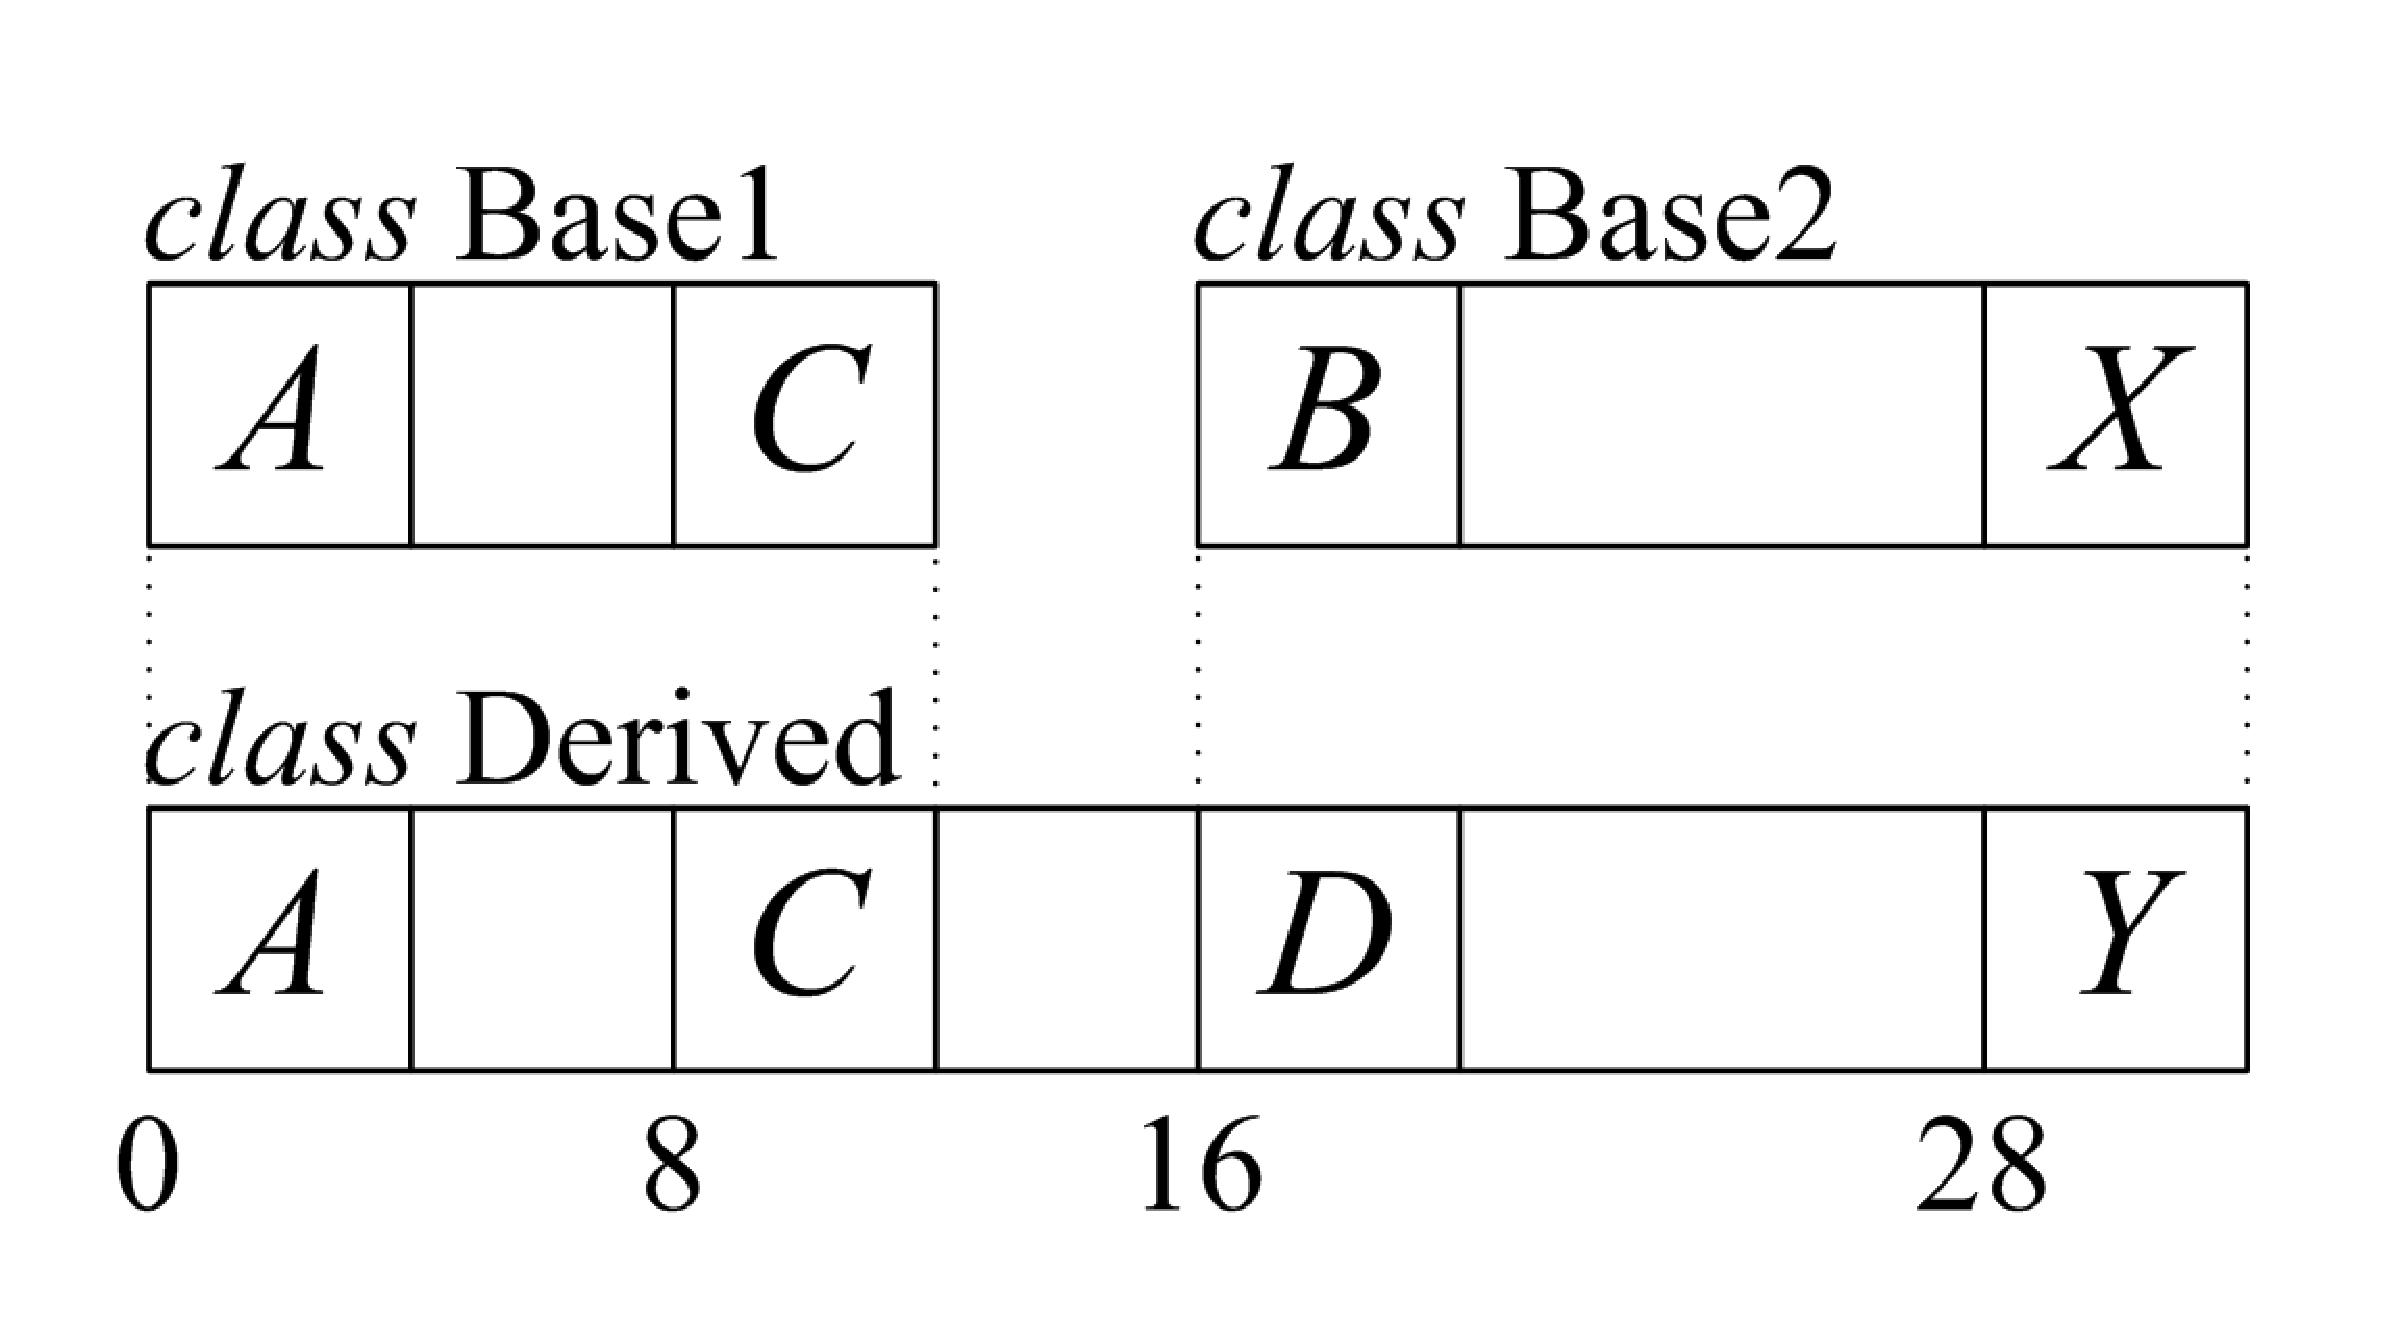
\includegraphics[width=4.9cm]{images/multiple}
\caption{Example of base class matching. Here $B$ is a direct base of $D$ and $X$ is a direct base of $Y$.}
\label{fig:multiple}
\end{figure}

After a set of classes is constructed, inheritance relation inference
is performed.
For each class a set of possible direct base classes is constructed.
Class \lstinline{Base} can be a direct base of class \lstinline{Derived}
if it can be ``placed'' inside class \lstinline{Base} so that overlapping
vtables are either equal or connected by direct inheritance.
See fig.~\ref{fig:multiple} for an example.

Normally, there exists only one way to ``cover'' a class with
base classes. In case there are several coverings, then the one with
the largest number of vtables being equal to the vtables of the
class at hand is selected. If there are several such coverings,
the case is reported to the user. % zero reports so far

As a result,
direct base classes with offsets to the corresponding instances,
constructors, destructors, and vtables
are reconstructed for each class in a program.





\section{Implementation and experimental results}\label{sectionExperiments}
Presented methods have been implemented as a plugin
for IDA Pro interactive disassembler. The plugin is available for
download at \url{http://decompilation.info}.

The plugin has been tested on a variety of open-source software written in C++.
The process used is as follows.
First, the program is compiled with optimizations and RTTI and
RTTI-aware class hierarchy reconstruction algorithm is used to collect information
on polymorphic class hierarchy.
The program is then recompiled with optimizations and debug information but without RTTI.
Class hierarchy reconstruction algorithm that does not use RTTI structures is applied, and
debug information is used to restore the correspondence between vtables and actual polymorphic classes.
Results of the two class hierarchy reconstruction algorithms are then compared.

\begin{figure}[htb!]
\begin{tabular}{| l | r | r | r |}
\hline
Application &         doxygen & Shareaza & Notepad++ \\
\hline
Running time &          7.9s  &   18.9s  & 0.7s \\
\hline
Vtables found &         415   &   1128   &  95 \\
\hline
Vtable mismatches &     8.6\% &    4.1\% & 4.0\% \\
\hline
Classes found &         401   &   1108   &  95 \\
\hline
Non-classes &           0.9\% &    0.6\% &   0\% \\
\hline
Class mismatches &      9.7\% &    6.5\% & 10.5\% \\
\hline
\end{tabular}
\caption{Test results.}
\label{fig:tests}
\end{figure}

Test results
%for doxygen (source code documentation generator),
%Notepad++ (text editor) and Shareaza (peer-to-peer file sharing client)
are presented on fig. \ref{fig:tests}.
Tests were performed on a Core2Duo CPU at 2.8Ghz.

For each of the analyzed applications all vtables present in
the assembly have been found, and no false positives were registered.
``Vtable mismatches'' refer to vtables with reconstructed parent vtable differing
from the real one.
``Non-classes'' refer to reconstructed classes that were not present
in the source program.
``Class mismatches'' refer to classes with associated vtables or parents
reconstructed differently from the real ones.

All non-classes were created as a result of allocating several polymorphic
classes on the stack, where they were treated as a single class.

In some of the considered
mismatch cases the mismatch was caused by violation of one of presumptions
the algorithm relies on (such as usage of virtual inheritance).

Most of vtable mismatch cases were registered in classes with no data members
and no actions performed in constructors and destructors.
Hierarchies of such classes can be rearranged in virtually any way
without changing the semantics of the program.
That's why such mismatches are not actual errors.

Most of class mismatches were registered as a result of one class
including the other as a field.
As it was denoted in chapter \ref{chapterMultiple}, inheritance and inclusion
as a field are normally indistinguishable. That's why such mismatches
do not lead to misinterpretation of program semantics.

To further decrease the
mismatch rates, additional analysis is required, such as dynamic analysis
and deeper analysis of the actions performed in constructors and destructors.




\section{Conclusion and further work}
A method for automatic reconstruction of polymorphic class hierarchies
from assembly code obtained by compiling a C++ program is presented.
If the source C++ program is compiled with run-time type information enabled,
then the class hierarchy is reconstructed exactly in the same form as it
was in the source code.

If RTTI is not compiled into the assembly, reconstruction
method is based on the analysis of virtual function tables, constructors and destructors.
First, inheritance relation on a set of virtual tables is reconstructed using
the analysis of virtual function tables and virtual function table accesses.
Then additional analysis of constructors and destructors is used to restore
classes and relations between them. Multiple inheritance is handled
correctly.

Proposed methods were implemented as a plugin for IDA Pro interactive disassembler,
which is available for download.
The plugin has been tested on a variety of open-source software written in C++
showing low mismatch rates.

Directions for future work include
%deeper analysis of constructors
%and destructors to further increase the accuracy of class hierarchy
%reconstruction, as well as
reconstruction of exception handling blocks and other C++ features.
The main goal is to develop several techniques that could be implemented
as a set of tools for reconstructing low-level programs into C++
programming language.




\bibliographystyle{IEEEtran}
\bibliography{article}

\end{document}

% Local variables:
%  compile-command: "dopdf.bat"
% End:

